\subsubsection{Overall performance improvement}

We performed 91 experiments on 512, 1024, 2048 and 4096 nodes of Mira. The average improvement on 512 nodes for OPT and HEU were 50.63\% and 29.98\% respectively. On 1024 nodes, OPT and HEU showed 67.32\% and 27.61\% improvements respectively. 
%Over 91 experiments, the improvement averages for (Optimization, Heuristics)  are (50.63\%, 29.98\%) in 512-node partition, (67.32\%, 27.61\%) at 1024-node partition, (45.38\%, 18.32\%)) at 2048-node partition and (43.81\% and 13.20\%) at 4096-node partition. The 
Figure \ref{fig:alltests_1k} shows the overall performance of Optimization, Heuristics and MPI\_Alltoallv from 91 experiments on 2048-node partition. For this, OPT and HEU showed 45.38\% and 18.32\% improvement over MPI on average.
\begin{figure}[!htb]
\vspace{-0.15in}
\centering
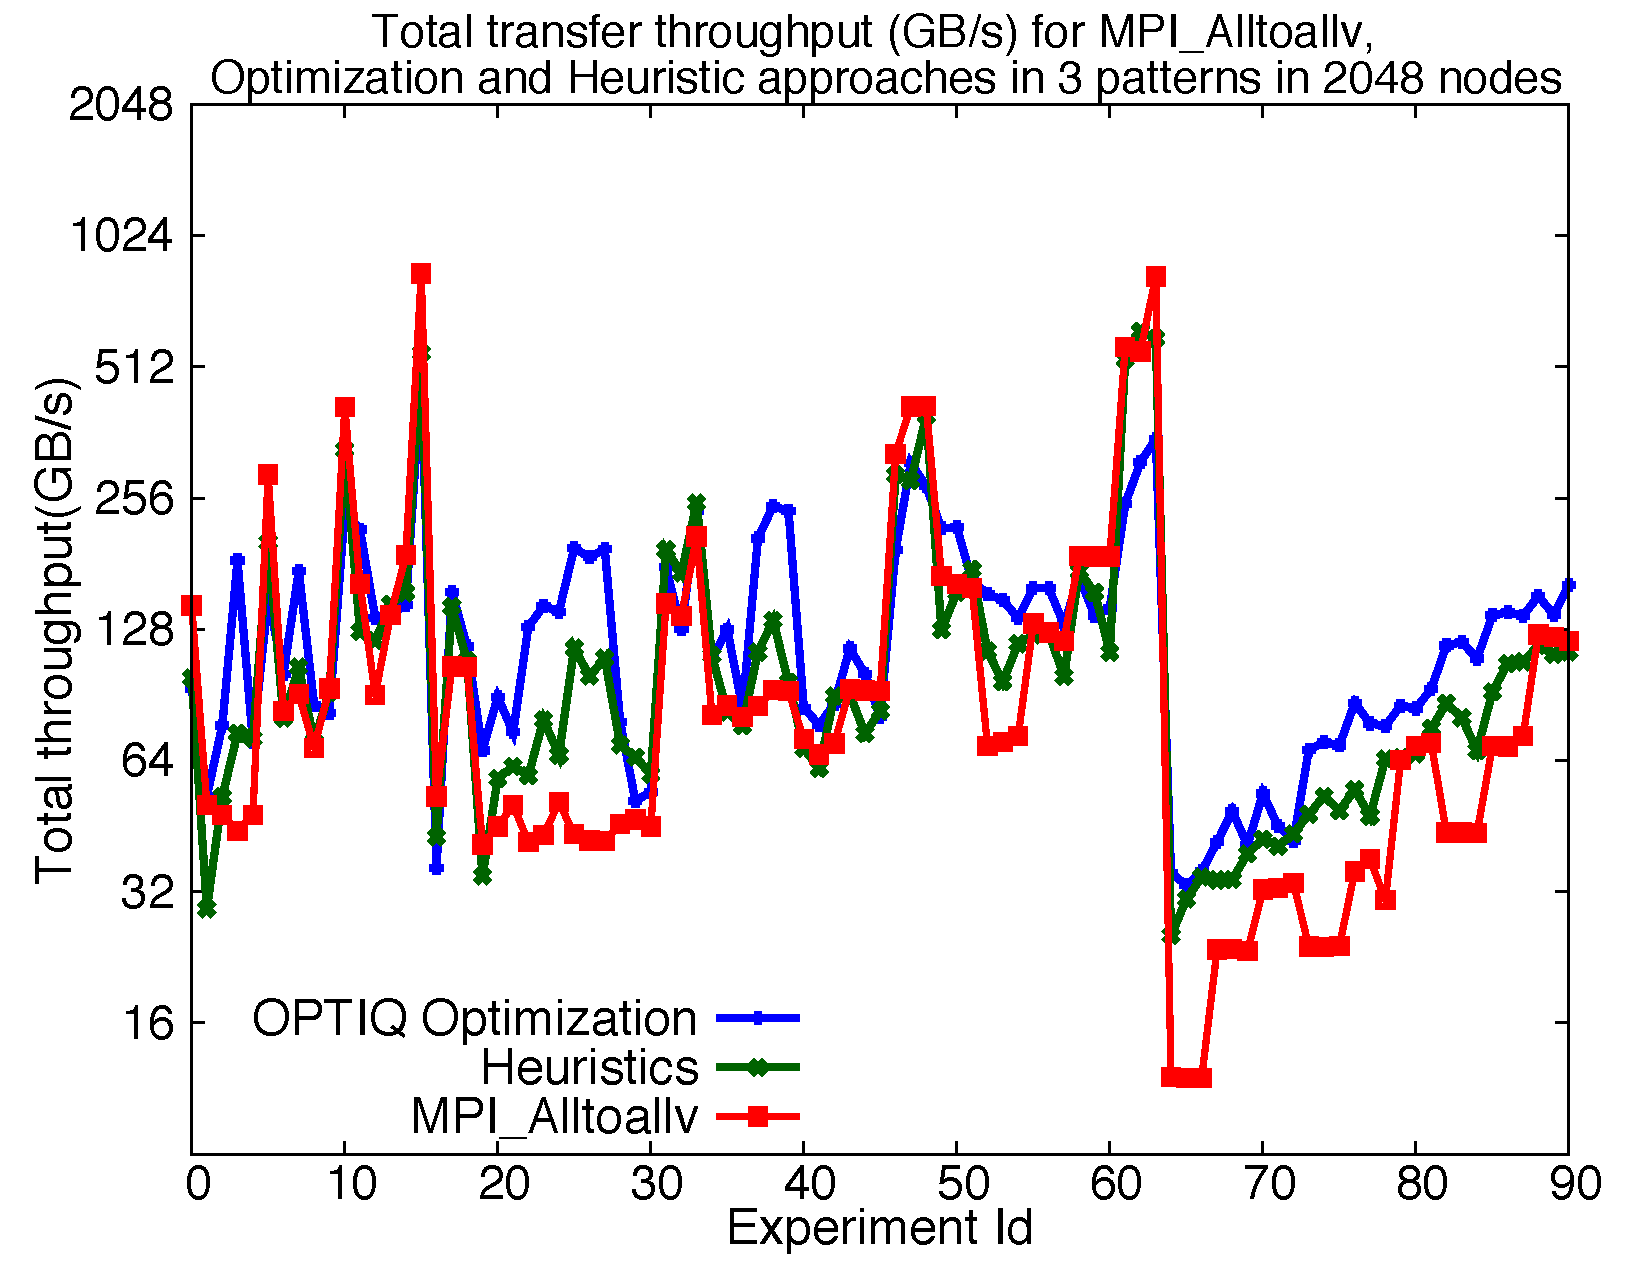
\includegraphics[scale=0.27]{figures/alltests_1k.pdf}
\vspace{-0.15in}
\caption{\small Total throughput from 91 cases for 3 patterns in 2048-node partition.}
%\caption{Total throughput from 91 cases for 3 patterns in 1024-node partition.} %you have 2048 in the figure title??!
\vspace{-0.15in}
\label{fig:alltests_1k}
\end{figure}
